\documentclass{article}
\usepackage[utf8]{inputenc}
\usepackage[english]{babel}
\usepackage{amsthm}
\usepackage{amssymb}
\usepackage{mathcomp}
\usepackage{amsmath}
\usepackage{natbib}
\usepackage{array}
\usepackage{wrapfig}
\usepackage{multirow}
\usepackage{tabularx}
\usepackage{graphicx}
\usepackage{geometry}
\usepackage{multicol}
\usepackage{blindtext}

\title{Homework 5}
\author{Sean Eva}
\date{April 2022}

\begin{document}

\maketitle

\section{Theoretical Problems}
\begin{enumerate}
    \item [12.6: Exercise 1. ]
    
    \begin{enumerate}
        \item 
        
        12.18 states: $\frac{1}{|C_k|}\sum_{i, i'\in C_k}\sum_{j=1}^p(x_{ij}-x_{i'j})^2 = 2\sum_{i\in C_k}\sum_{j=1}^p(x_{ij}-\bar{x}_{kj})^2$
        \begin{proof}
        We may write $\frac{1}{|C_k|}\sum_{i, i'\in C_k}\sum_{j=1}^p(x_{ij}-x_{i'j})^2 = \sum_i\sum_jx^2_{ij}-2\sum_i\sum_jx_{ij}\bar{x}_kj + \sum_i\sum_jx^2_{ij} = 2\sum_i\sum_jx^2_{ij}-2|C_k|\sum_j\bar{x}^2_{kj}$ which implies that $2\sum_i\sum_jx^2_{ij}-4\sum_i\sum_jx_{ij}\bar{x}_{kj} + 2\sum_i\sum_j\bar{x}^2_{kj} = 2\sum_i\sum_jx^2_{ij}-2|C_k|\sum_j\bar{x}^2_{kj}.$ Which therefore proves 12.18 as desired.
        \end{proof}
        
        \item
        
        This identity shows us that when we assign each observation to the cluster whose centroid is closest, we actually decrease the right member of the identity. So, we also will decrease the left member of the identity which is our objective. Another way of seeing this is that the identity shows that minimizes the sum of the squared Euclidean distance for each cluster is the same as minimizing the within-cluster variance for each cluster.
        
    \end{enumerate}
    
    \item [12.6: Exercise 3. ]
    
    \begin{enumerate}
        \item 
        
        Graph with points:
        \begin{center}
            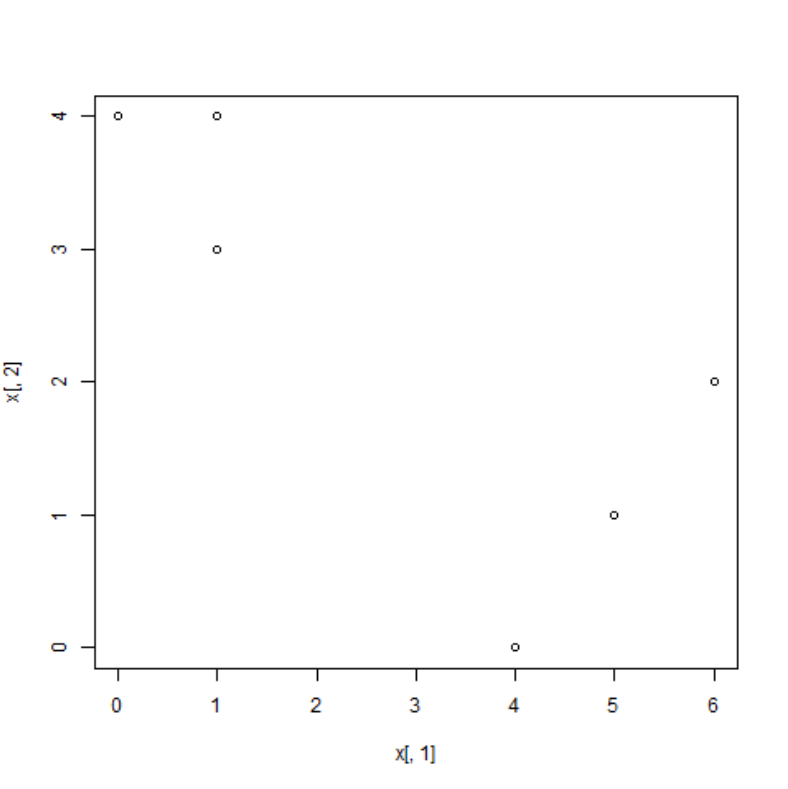
\includegraphics[width=8cm]{HW5_2_a.png}
        \end{center}
        
        \item
        
        Cluster 1: Points 1, 2, 5. Cluster 2: 3, 4, 6.
        \begin{center}
            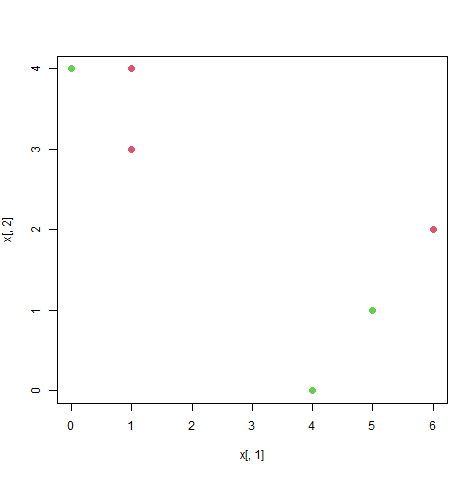
\includegraphics[width=8cm]{HW5_2_b.png}
        \end{center}
        
        \item
        
        Calculation: \\
        $\bar{x}_{11} = \frac{1}{3}(1+1+6) = \frac{8}{3}, \bar{x}_{12} = \frac{1}{3}(2+4+3) = 3.$\\
        $\bar{x0}_{21} = \frac{1}{3}(0+4+5) = 3, \bar{x}_{22} = \frac{1}{3}(4+0+1) = \frac{5}{3}$\\
        On graph marked with x's.
        \begin{center}
            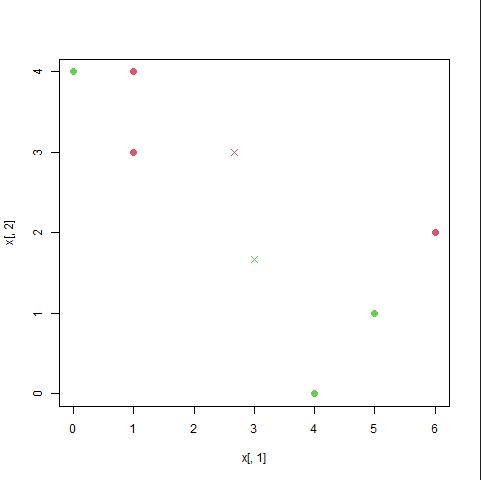
\includegraphics[width=8cm]{HW5_2_c.png}
        \end{center}
        
        \item
        
        Cluster 1: Points 1, 2, 3. Cluster 2: 4, 5, 6.
        New graph with reassigned locations.
        \begin{center}
            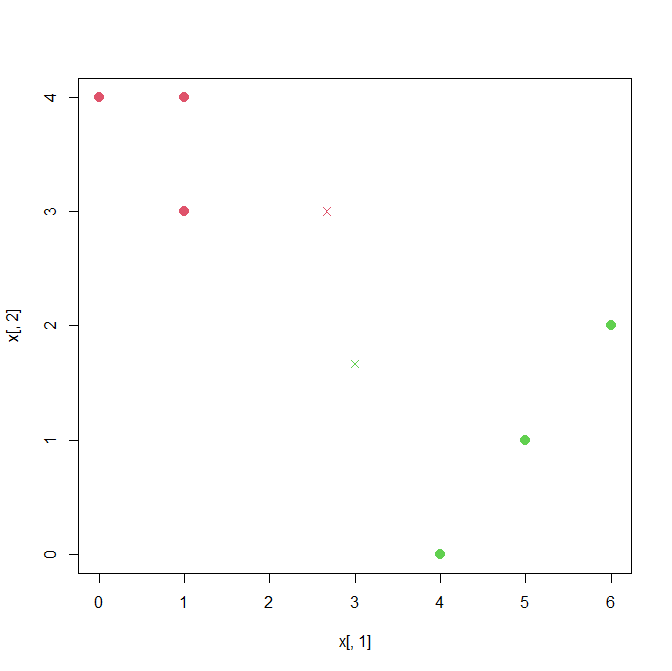
\includegraphics[width=8cm]{HW5_2_d.png}
        \end{center}
        
        \item
        
        New Calculations:\\
        $\bar{x}_{11} = \frac{1}{3}(1+1+0) = \frac{2}{3}, \bar{x}_{12} = \frac{1}{3}(4+3+4) = \frac{11}{3}$\\
        $\bar{x}_{21} = \frac{1}{3}(5+6+4) = 5, \bar{x}_{22} = \frac{1}{3}(1+2+0) = 1$\\
        If we reassign and perform again we will arrive to the same centroids and groupings again so the process will end here. New graph with new centroid locations:
        \begin{center}
            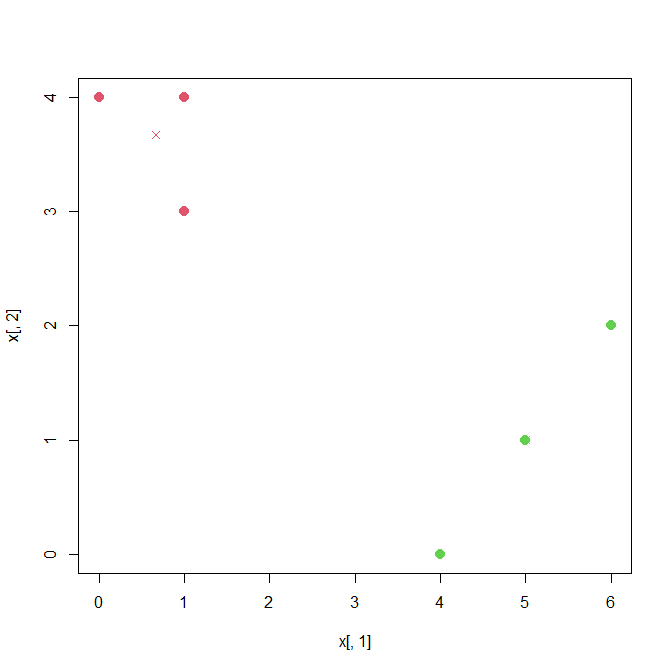
\includegraphics[width=8cm]{HW5_2_e.png}
        \end{center}
        
        \item
        
        Graph with final labels.
        \begin{center}
            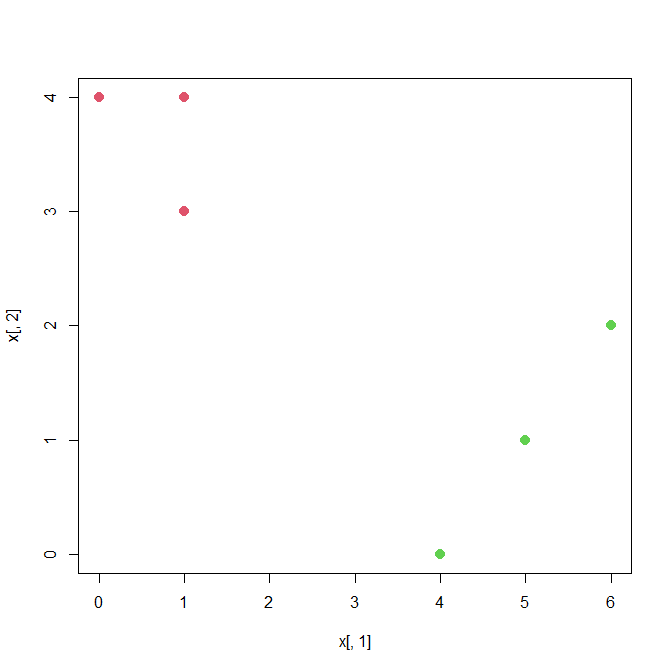
\includegraphics[width=8cm]{HW5_2_f.png}
        \end{center}
        
    \end{enumerate}
    
    \item [n-complete graph: ]
    
    \begin{enumerate}
        \item [1. ]
        
        $\begin{bmatrix}
        n-1 & -1 & -1 & \cdots & -1\\
        -1 & n-1 & -1 & \cdots & -1\\
        \vdots & \vdots & \vdots & \ddots & -1\\
        -1 & -1 & -1 & \cdots & n-1
        \end{bmatrix}$
        
        \item [2. ]
        
        The eigenvalues are $\lambda = 0, n$ where $n$ has a geometric multiplicity of $n-1$. The eigenvector corresponding to $\lambda = 0$ is 
        $\begin{bmatrix}
        1\\
        1\\
        \vdots\\
        1
        \end{bmatrix}$
        and the eigenvectors corresponding to $\lambda = n$ are 
        $\begin{bmatrix}
        -1\\
        1\\
        0\\
        \vdots\\
        0
        \end{bmatrix}, 
        \begin{bmatrix}
        -1\\
        0\\
        1\\
        \vdots\\
        0
        \end{bmatrix}, ..., 
        \begin{bmatrix}
        -1\\
        0\\
        0\\
        \vdots\\
        1
        \end{bmatrix}$.
        
    \end{enumerate}
    
\end{enumerate}

\section{Programming}
\begin{enumerate}
    \item [1. ]
    
    \begin{enumerate}
        
        All in coding file.
        
    \end{enumerate}
    
    \item [2. ]
    
    Sorry I ran out of time on this question.
    
\end{enumerate}

\end{document}
